\chapter{Especificações e Arquitetura do Sistema}
\label{chap:arquitetura}
Durante todo o desenvolvimento do sistema, buscou-se não se utilizar dos modelos de arquitetura comumente empregados neste tipo de aplicação, que trabalham com grandes volumes de dados, um dos motivos vem a ser pela grande complexidade encontrada ao se trabalhar com módulos Apache como o Hadoop Common, Hadoop Distributed File System (HDFS), Hadoop YARN e Hadoop MapReduce, os quais dependendo de suas aplicações acabam por gerar dependências de outras ferramentas como Cassandra, Spark, ZooKeeper, entre outras que se mostram apesar de robustas, muito complexas e com uma curva de aprendizagem alta demais para serem usadas de imediato.

Outro motivo de grande valor para o desenvolvimento de uma nova arquitetura tem sido a empregabilidade de novas ferramentas utilizadas no lado \textit{backend}, por assim dizer, relacionado a organização dentro dos servidores, conceitos de desenvolvimento e bancos de dados que tem ganhado força dentro do mercado e se mostradas bem aplicáveis em projetos com grandes volumes de dados e alta disponibilidade, além de possuir uma baixa curva de aprendizagem, se comparadas com as tecnologias tradicionais.

\section{Micro Serviços}
\label{sec:microserviços}
Os Micros Serviços tem se tornado um padrão de projeto muito utilizado em aplicações de multiplataforma, pois através deste padrão este tipo de aplicação tem se tornado mais fácil de se desenvolver, demandando menos tempo. A ideia do padrão de Micro Serviços é desenvolver pequenos serviços autônomos que trabalham juntos, ou seja, um serviço possui uma única responsabilidade bem definida, mas para o funcionamento da aplicação por completa é necessário o uso de todos os serviços disponíveis dentro do domínio da aplicação. Considerando que um serviço venha a ser um \textit{endpoint} de uma \textit{Application Programming Interface} (API), que pode informações como todos os dados de uma tabela.~\cite{newman2015building}

%A escolha do desenvolvimento neste padrão se deve ao fato de ser fácil escalável e ter um grande reaproveitamento de código, sem contar o paralelismo na execução de tarefas

\section{Docker}
\label{sec:docker}
O Docker é uma plataforma aberta criada com o intuito de tornar mais ágil o desenvolvimento, implantação e execução de aplicações em ambientes isolados, além de ser multiplataforma, tudo isso através do conceito de conteinerização e imagens, em que numa imagem se tem todos os arquivos necessários para a criação de um contêiner, este por sua vez, possui a aplicação encapsulada  e funcionando.

Desta forma se tem uma grande flexibilidade para trabalhar com as aplicações, pois estas irão funcionar tanto em um notebook, quanto em um mainframe. Este conceito de contêiner se assimila ao processo de criação de máquinas virtuais, onde se tem todo o sistema operacional virtualizado, já o Docker realiza uma virtualização á nível do sistema operacional, mantendo um único kernel no \textit{host} executando processos (contêineres) de forma isolada, isso é possível através do uso de \textit{namespaces}, fazendo com que um processo só tenha acesso a recursos de outro se isso for explicitamente configurado na criação dos ambientes. Para que não ocorra a exaustão de recursos no \textit{host} o Docker se utiliza de \textit{cgroups} do kernel, responsável por criar limites de hardware para os processos, evitando o uso exagerado de recursos por apenas um processo. A figura \ref{fig:arqdocker} apresenta a organização a nível de sistema operacional de um \textit{host} utilizando Docker.~\cite{docker}

\begin{figure}[!h]
\caption{\label{fig:arqdocker} Arquitetura Docker}
\begin{center}
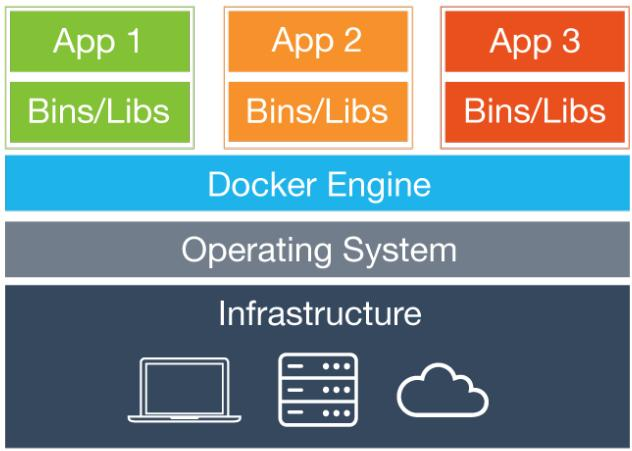
\includegraphics[scale=0.3]{arqdocker}
\end{center}
\legend{Fonte: \citeauthor{docker}, \citeyear{docker}} 
\end{figure}

O Docker tem ganhado fama no mercado, principalmente pelos profissionais de infraestrutura, pois ele tem facilitado o trabalho destas pessoas, fazendo com que elas economizem tempo para realizar a instalação de um software, não necessitando mais se preocupar com todas as dependências e ferramentas necessárias para o funcionamento do software, basta apenas se utilizar uma imagem da aplicação e transformá-la em um contêiner em qualquer ambiente que se esteja.

\subsection{Docker Compose}
Com o aumento da complexidade do ambiente em que se está hospedada a aplicação, surgem as necessidades de se criar mais contêineres, tornando o seu gerenciamento um tanto quanto complicado, é neste cenário que se aplica o Docker Compose, uma ferramenta que trabalha juntamente com o Docker, ele se caracteriza por definir e executar múltiplos contêineres, pois através do uso de um arquivo que descreve todos os contêineres e configurações necessárias para o funcionamento de uma aplicação por completa, como pode ser visto um exemplo deste arquivo na figura \ref{fig:arqdockercompose}, o Docker Compose tem a capacidade de criá-los, reiniciá-los e desligá-los quando necessário, facilitando assim o uso de contêineres.

\begin{figure}[!h]
\caption{\label{fig:arqdockercompose} Arquivo Docker Compose}
\begin{center}
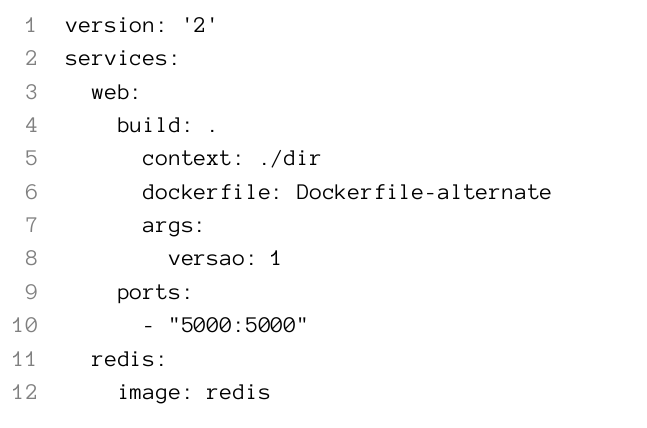
\includegraphics[scale=0.5]{arqdockercompose}
\end{center}
\legend{Fonte: \citeauthor{docker}, \citeyear{docker}} 
\end{figure}

\subsection{Docker Swarm}
Balanceamento entre contêineres

\section{Redis}
\label{sec:redis}
Redis é um banco de dados No-SQL destinado ao armazenamento em memória de dados no tipo chave-valor, utilizado para manter cache das aplicações, nesse cache podem ser armazenados \textit{hashs}, \textit{strings}, \textit{bitmaps}, listas e \textit{Hyperloglogs}, estes dados tem uma data de expiração após serem persistidos no Redis, por ser um banco de dados em memória, as ações de escrita e leitura se tornam mais rápidas do que uma leitura ou escrita em disco, dando maior \textit{performance} ás aplicações nas quais ele é implantado.~\cite{da2015redis}

\section{Tecnologias}
\label{sec:tecnologias}
Mostrar de forma específica cada tecnologia que será empregada

\subsection{Clojure}
Apresentar a linguagem de programação \textit{Clojure} e como ela é empregada no trabalho.

\subsection{Kafka}
Apresentar seu uso para realizar funções em tempo real dentro do sistema, bem como seu funcionamento.

\subsection{MongoDB}
Apresentar as características do banco NoSQL seu uso e diferenças entre um banco SQL, bem como seus pontos positivos.

\subsection{Datomic}
Apresentar uma nova forma de armazenar dados, se utilizando de histórico, sempre mantendo o estado anterior dos dados.

